\documentclass[12pt,a4paper,leqno]{report}

\usepackage[T1]{fontenc}
\usepackage[english]{babel}
\usepackage{amsthm}
\usepackage{amsfonts}
\usepackage{amsmath}
\usepackage{amssymb}
\usepackage{tikz}
\usepackage{listings}

\newcommand{\R}{\mathbb{R}}
\newcommand{\C}{\mathbb{C}}
\newcommand{\Q}{\mathbb{Q}}
\newcommand{\N}{\mathbb{N}}
\newcommand{\No}{\mathbb{N}_0}
\newcommand{\Z}{\mathbb{Z}}
\newcommand{\diam}{\operatorname{diam}}

\theoremstyle{plain}
\newtheorem{equa}[equation]{Equation}
\newtheorem{lem}[equation]{Lemma}
\newtheorem{prop}[equation]{Proposition}
\newtheorem{cor}[equation]{Corollary}

\theoremstyle{definition}
\newtheorem{defi}[equation]{definition}
\newtheorem{conj}[equation]{Conjecture}
\newtheorem{example}[equation]{Example}

\theoremstyle{remark}
\newtheorem{note}[equation]{Note}

\pagestyle{plain}
\makeatletter
\renewcommand{\@seccntformat}[1]{}
\makeatother
\setcounter{page}{1}
\addtolength{\hoffset}{-1.15cm}
\addtolength{\textwidth}{2.3cm}
\addtolength{\voffset}{0.45cm}
\addtolength{\textheight}{-0.9cm}

\graphicspath{ {../figures/} }

\title{Data Analytics 2 - Product Type Sales Prediction}
\author{Tuomo Kareoja}
\date{}

\begin{document}

\maketitle

\begin{table}[h!]
  \begin{center}
    \begin{tabular}{l|c|r}
      \textbf{Version Number} & \textbf{Changes} & \textbf{Date} \\
      \hline
      0.9 & Basic layout & 02.09.2019\\
      1.0 & Finished Report & 03.09.2019\\
    \end{tabular}
  \end{center}
\end{table}

\newpage

\section{Predicted Sales for New Laptops, Smartphones, Netbooks}

We predicted the sales volume for future products in the categories Laptops,
PCs, Smartphones and Netbooks. Below are the predicted volumes. One of the Netbooks
looks like a clear winner, but if we concentrate on the categories we see that
our new smartphones were predicted to perform well all around except for product 195.

\bigskip
{
    \centering
    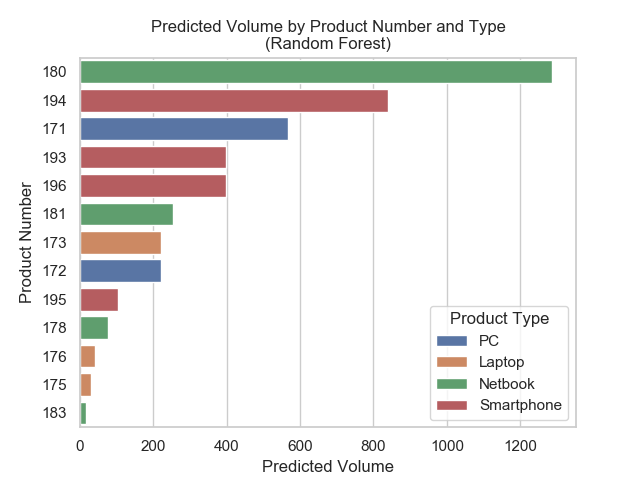
\includegraphics[width=\textwidth,height=\textheight,keepaspectratio]{predicted_volume_rf.png}
    \par
}
\bigskip

\section{Selected Model and It's Performance}

The model that was used to create these predictions was a Random Forest Model.
The model was trained using all the data in training set, except for the
Extended Warranties. This means that we used product categories as different
from our categories of interest as Printer Supplies and accessories.

Below are the predictions for volume in the training set. Included in the graph
are both the predictions made from by training with the whole dataset and the predicting
the values with this model (insample) and predictions made by training the model without
the observation that was predicted (outsample). The more reliable measure of the models
actual predictive power is the outsample error. We can see that the model is not very
good with products that have actual sales volumes of over 2000 and this is particularly
true for the outsample predictions. We also see that the outsample error is over twice that
of the insample error. This means that despite our efforts there is substantial overfitting
of the model to the train dataset.

\bigskip
{
    \centering
    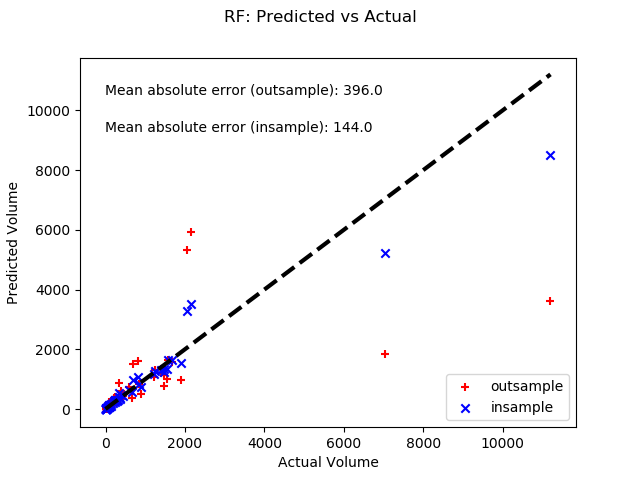
\includegraphics[width=\textwidth,height=\textheight,keepaspectratio]{predictions_final_rf.png}
    \par
}
\bigskip

As we in the end interested only in the models accuracy to in predicting the volumes
of PCs, Laptops, Smartphones and Netbooks, below is the same graph as before, but now
only showing products of these categories:

\bigskip
{
    \centering
    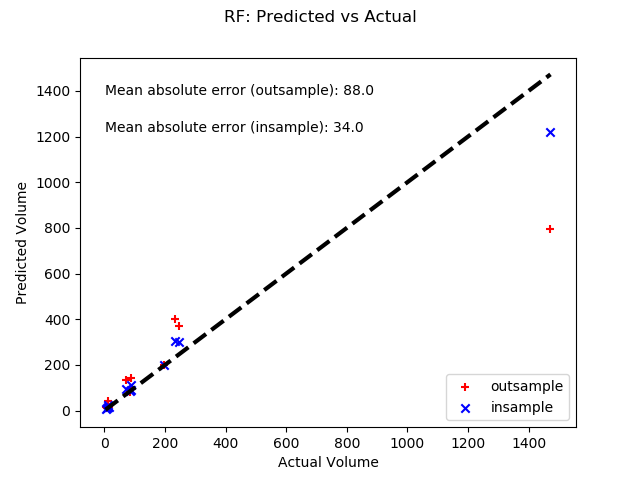
\includegraphics[width=\textwidth,height=\textheight,keepaspectratio]{predictions_final_lim_pred_rf.png}
    \par
}
\bigskip

The model seems to actually work quite good in this case, but we see the same problems of overfitting
and poor performance when the number of sales is high.

Out of curiosity we also tried to train the model on just Smartphones, PCs, Laptops and Smartphones.
This did not work out well. Even though conceptually it makes sense to use similar products for
predictions, the amount of data that we have was so small that the model is very unreliable.
Below is the familiar plot of the model predicting just product from our categories of interest:

\bigskip
{
    \centering
    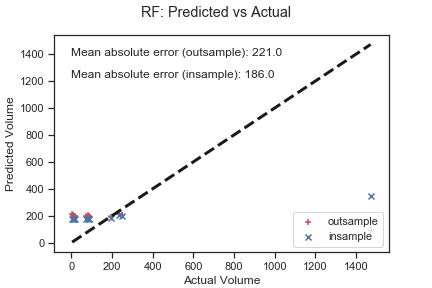
\includegraphics[width=\textwidth,height=\textheight,keepaspectratio]{predictions_best_lim_pred_train_rf.png}
    \par
}
\bigskip


\section{Relation of Reviews to Sales Volume}

On top of predicting with the model. We were asked to analyse the relation of the reviews
the to the sales volume. To do this we combined all the laptops, smartphones, PCs and Netbooks
from both the training data and the new products. Because the new products did of course
not have a sales volume, we used our predictions for these. We also did not use
all the review columns for our model as this made the model less accurate. The review columns
that were dropped were 5 star reviews and negative service reviews. 5 star reviews
were dropped because they had a perfect correlation with the volume and as this is
almost impossible in real life, the column was dropped as faulty. The negative service
reviews were dropped because they did not make the model any more accurate after
we added positive service reviews. These reviews seem to provide almost identical
information.

Here are the graphs for the relationship of the number of reviews to sales volume:

\bigskip
{
    \centering
    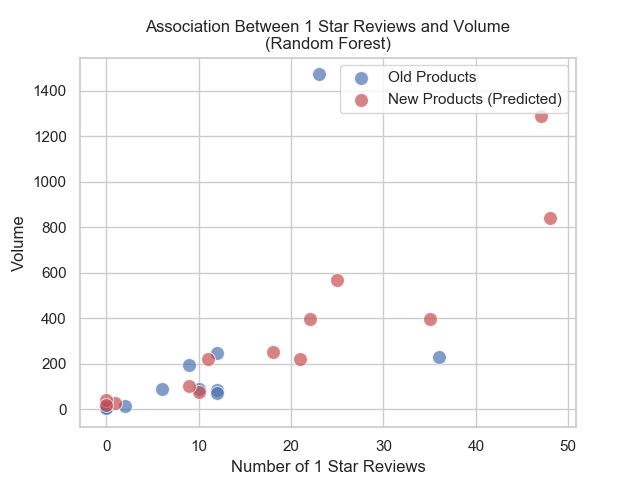
\includegraphics[width=\textwidth,height=\textheight,keepaspectratio]{volume_x1StarReviews_relation.png}
    \par
}
\bigskip

\bigskip
{
    \centering
    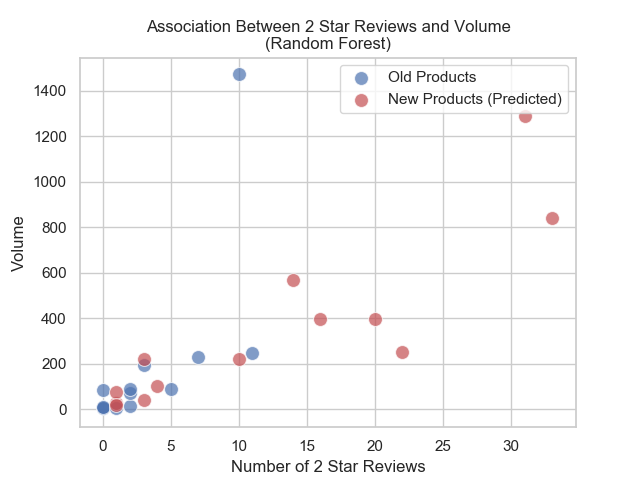
\includegraphics[width=\textwidth,height=\textheight,keepaspectratio]{volume_x2StarReviews_relation.png}
    \par
}
\bigskip

\bigskip
{
    \centering
    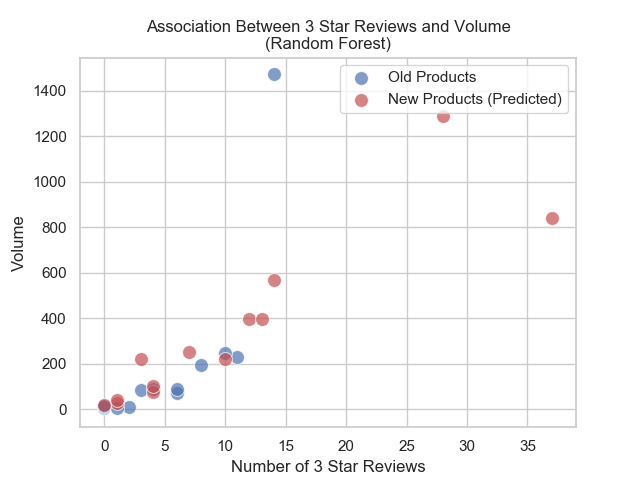
\includegraphics[width=\textwidth,height=\textheight,keepaspectratio]{volume_x3StarReviews_relation.png}
    \par
}
\bigskip

\bigskip
{
    \centering
    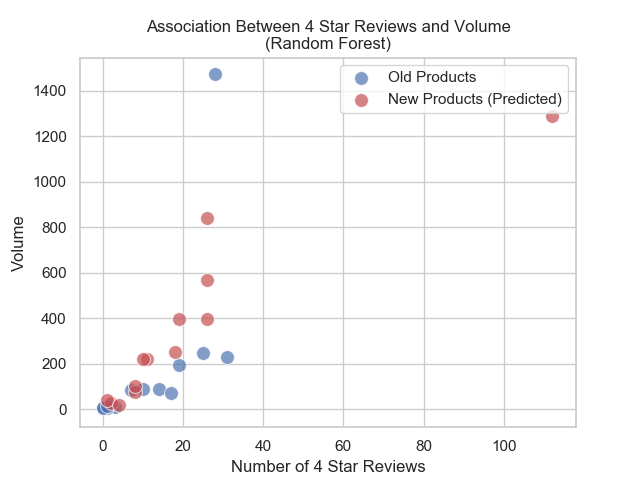
\includegraphics[width=\textwidth,height=\textheight,keepaspectratio]{volume_x4StarReviews_relation.png}
    \par
}
\bigskip

\bigskip
{
    \centering
    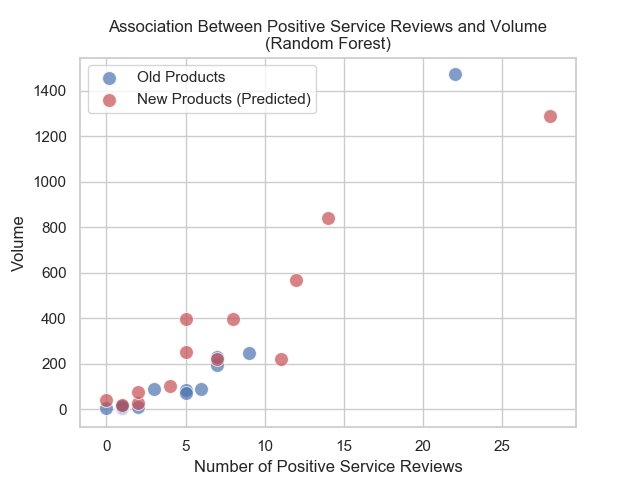
\includegraphics[width=\textwidth,height=\textheight,keepaspectratio]{volume_PositiveServiceReview_relation.png}
    \par
}
\bigskip

We can see that the relation is always positive so more reviews in itself
are related to larger sales amount even for low reviews. This relationship can be seen in both
the actual data volume and the predicted volume. It seems that the most
import information about the reviews is just their number and not their
message.


\section{Model Comparison and Performance}

Four models were considered for the predictions: K-nearest Neighbors (KNN)
Linear models, Support Vector Machines (SVM) and Random Forest. Below are graphs
of their performance without hyperparameter optimization and feature selection.

\bigskip
{
    \centering
    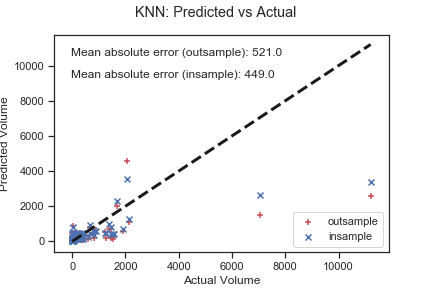
\includegraphics[width=\textwidth,height=\textheight,keepaspectratio]{predictions_unoptimized_simple_knn.png}
    \par
}
\bigskip

\bigskip
{
    \centering
    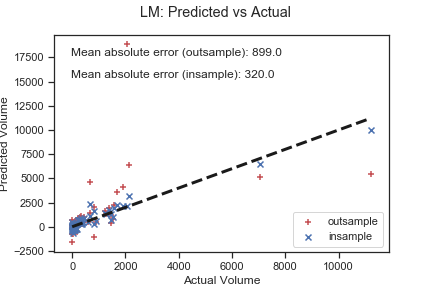
\includegraphics[width=\textwidth,height=\textheight,keepaspectratio]{predictions_unoptimized_simple_lm.png}
    \par
}
\bigskip

\bigskip
{
    \centering
    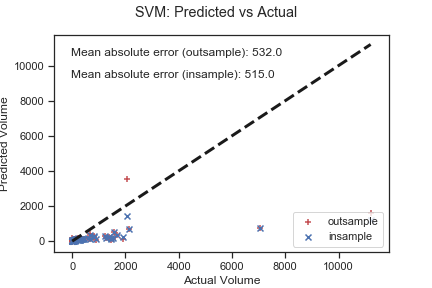
\includegraphics[width=\textwidth,height=\textheight,keepaspectratio]{predictions_unoptimized_simple_svm.png}
    \par
}
\bigskip

\bigskip
{
    \centering
    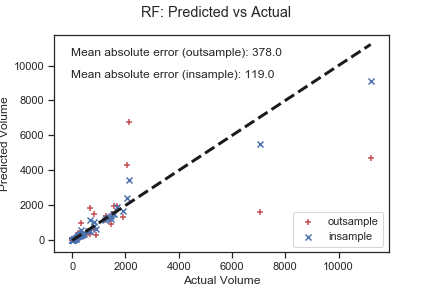
\includegraphics[width=\textwidth,height=\textheight,keepaspectratio]{predictions_unoptimized_simple_rf.png}
    \par
}
\bigskip

We can see that the random forest performed clearly the best, even though
it was clearly overfitting. SVM and KNN did not have the overfitting problem,
but were overall less accurate.

From these investigations KNN and SVM were dropped as their accuracy
was less than Random Forest and their interpretability is not very good.
Linear models were kept for further investigations although their results
were the worst, because it was thought that model could be improved much
with regularization and that its interpretability could prove interesting.
This was not to prove so as even with two steps of feature selection with
a separate linear model and applying L1 and L2 regularization with GLMNET
model, the performance remained poor. Further problem with the linear model
was that it was prone to give predictions for volume that were below 0. This
is almost and unavoidable problem for linear models when training data includes
volumes that are already very close to zero or even zero. Below you can see
the graph of the performance of the best linear model that we produced:

\bigskip
{
    \centering
    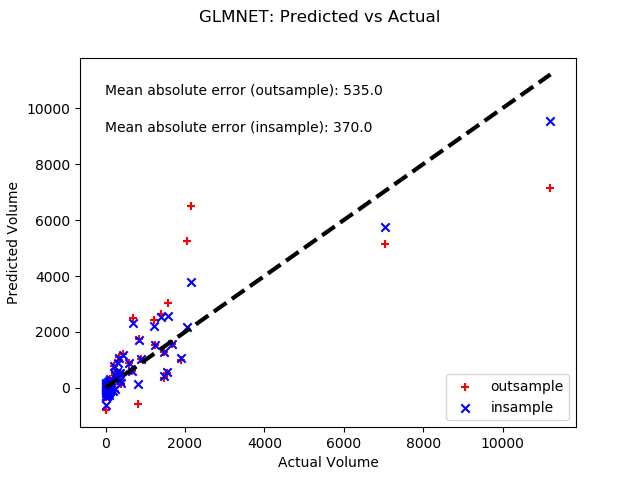
\includegraphics[width=\textwidth,height=\textheight,keepaspectratio]{predictions_final_glmnet.png}
    \par
}
\bigskip

Finally here are the results when limit predictions to the product
of our categories of interest:

\bigskip
{
    \centering
    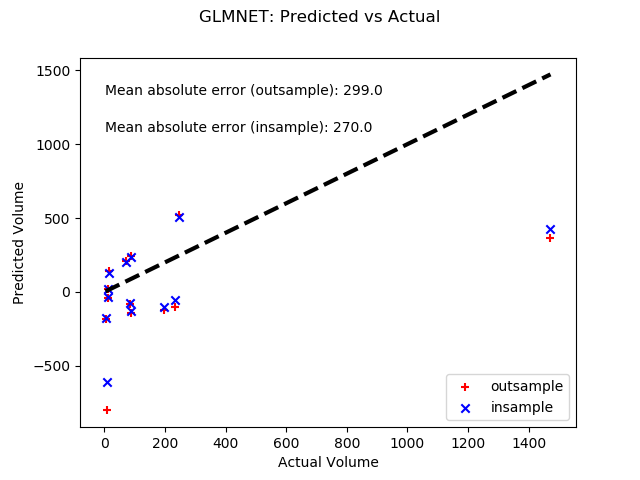
\includegraphics[width=\textwidth,height=\textheight,keepaspectratio]{predictions_final_lim_pred_glmnet.png}
    \par
}
\bigskip

\end{document}
